% !Mode:: "TeX:UTF-8"
% !TEX program  = xelatex
%\documentclass{cumcmthesis}
\bibliographystyle{plain}
\documentclass[withoutpreface,bwprint]{cumcmthesis} %去掉封面与编号页
\usepackage{verbatim}
\usepackage{url}
\usepackage{cite}
\usepackage[numbers,sort&compress]{natbib}
\title{基于决策树与概率控制优化模型下的机场出租车问题分析}
\tihao{C}
\baominghao{201931001025}
\schoolname{}
\membera{}
\memberb{}
\memberc{}
\supervisor{}
\yearinput{}
\monthinput{}
\dayinput{}

\begin{document}

 \maketitle
 \begin{abstract}
本文主要探究了如何在机场乘客数量变化规律以及出租车司机收益的影响下,建立出租车司机决策模型。并通过建立基于数据挖掘算法的决策树模型来为出租车司机提供较为科学合理的选择建议,使其在等待载客与直接放空返回市区拉客两种选择中做出可使自身经济效益最大化的决策。同时通过建立出租车上客区通行能力配置与概率控制优化模型以及排队模型,为相应管理部门合理规划“上车点”的最优数量,并给出一个可促使出租车收益均衡的“优先”安排方案。

针对问题一,可通过计算不纯度度量对选取属性的纯度进行检验,并计算其信息增益率以证明排队等待时长,目的地距离,市区载客时长以及时段等属性选取的合理性。由此建立决策树模型,通过比较“等待载客”与“直接放空返回市区拉客”两种状态下司机处于不同等待时长时的预期收益来做出使其效益最大化的决策。

针对问题二,筛选发车地点位于北京市首都国际机场内的出租车的行车轨迹数据,整理出其行车距离,并运用出租车收费软件计算出相应的司机收益。同时根据整理的数据计算出乘车目的地为远,中,近三类距离的发生概率,使用决策树计算方法得出这三类情况下的收益真实值并进行比较。其后通过Gini值验证样本选取的合理性,通过决策树分类模型的评分函数,验证决策树模型建立的合理性。

针对问题三,建立出租车上客区通行能力配置与概率控制优化模型,并通过计算得到双车道出租车上客区的通过能力表,由表可知,当车道为双车道时,上客口数量应控制在8-11个,此时双方的效益基本达到了平衡,在一定程度上实现了最优。

针对问题四,建立多服务台泊松到达,负指数服务时间,系统容量有限制的排队模型。根据出租车进站与离站时间以及根据GPS行车轨迹确定的行车里程对是否给予“优先权”进行判断。并使用出租车排队管理系统综合时间长度与行车里程对返回机场的出租车进行统计分析,从而筛选出用于衡量是否给予返回出租车优先权的指标体系。 \\ \\ \\

\keywords{决策树\quad   挖掘算法\quad  概率控制优化模型\quad 排队模型}
\end{abstract}

%目录
%\tableofcontents

%\newpage

\section{问题重述}  
城市出租车以其便利、快捷、舒适的优势,在城市居民的日常出行中发挥着巨大的作用。特别是在是城市人口规模急速扩大和社会活动多元化程度日益加深的今天,出租车行业的市场需求更是有增无减。根据交通运输部发布的数据,2010-2018年间,全国出租汽车运送旅客保持在340亿人次以上;2010-2016年,全国城市出租车辆规模保持逐年增长,年复合增长率为2.35$\%$。
同时,随着我国经济技术的持续发展和社会制度的不断进步,越来越多的城市正面临着由 大量的客运吞吐量多带来的一系列问题。其中,机场出租车送客后的决策问题引起社会 各界的广泛关注。出租车司机或选择进入机场特定的“蓄车池”,按照“先来后到”的顺序进行排队等待;或选择直接返回市区载客,但此选择将会使司机面临较高的空载成本,也可能丧失部分潜在收益。并且,机场客运量也与季节、时段和地区旅游业等因素有关。基于此类社会需要,我们需要对以下问题进行研究:

问题一:对影响出租车司机决策的相关原因进行探讨,并讨论其作用方式,特别是人流量与司机收益两种因素的变化对于司机决策的影响,建立相关模型并给出符合司机切实利益的决策。

问题二:收集我国某城市机场出租车流量的实际数据,在进行数据整理与筛选后代入模型进行计算,从而提供适用于该机场司机的决策,并就模型的合理性与相关因素的相关性进行探讨。

问题三:在机场经常会出现乘客与空车无法高效对接的情况。要求在双车道的情况下为管理部门提供合理的“上车点”数量,以提高双方效率。

问题四:乘客目的地与机场的距离决定了司机的收入,为平衡司机们的收益,避免其在长时间等待后却接到短途客人造成亏损的状况,如何合理赋予短途载客返回的司机“优先权”。
\section{模型的假设}
\begin{enumerate}
	\item 假设出租车司机可以根据在上客口等待载客的车队长度以及乘客数量变化规律判断出等待时长;
	\item 假设出租车司机在任何时段均按照城市出租车收费标准收取费用;
	\item 假设天气,节假日等因素均不在在考虑范围内;
	\item 假设机场载客的出租车不存在拼车的情况,排除拼车对司机收益的影响。
\end{enumerate}

\section{符号说明}
\begin{center}
	\begin{tabular}{cc}
		\hline
		\makebox[0.3\textwidth][c]{符号}	&  \makebox[0.4\textwidth][c]{意义} \\ \hline
		$P_0$	    & 闲置状态的概率\\ \hline
		Lq	    & 排队的平均乘客数量\\ \hline
		L     & 正在上车的乘客数量\\ \hline
		Wq     &  每位乘客的平均等待时间\\ \hline
		Ws	    & 司机的平均返回时间\\ \hline
		Pw	    & 乘客需排队等待的概率\\ \hline
		I	    & 为不纯度的度量\\ \hline
		N   & 划分后的个数\\ \hline
		Delta	    & 信息增益\\ \hline
		c   & 为车站设置的上客口的数量\\ \hline
		$\lambda \mathrm{n}$   & 乘客的到达率\\ \hline
		$\rho$   & 服务强度\\ \hline
		$\mu_{n}$   & 出租车的服务率\\ \hline
		
	\end{tabular}
\end{center}

\newpage
\section{问题分析}
\subsection{问题一的分析}
为了建立出租车司机的选择决策模型,作者需要提炼出影响出租车司机的主要决策因素,并且分析出相关因素的影响机理,从而给出符合出租车司机在不同时段,不同状况下的实际需求的选择策略。

可根据题设中对于出租车司机选择的限定将其选择划分为在上客口等客或空载返回两种情况,且在出租车司机可以根据在上客口等待载客的车队长度以及乘客数量变化规律判断出等待时长的前提下,将司机等待时长合理划分为连续区间。因为出租车司机将乘客送达目的地后的实际里程数存在差异,即乘客目的地距离机场的距离会导致出租车司机的收入差异,所以可将乘客目的地距机场的里程划分为远程,中程,近程三类,并以此为根据获得三类情况下出租车司机损益的观测值。从而根据不同等待时长下乘客目的地与机场距离远,中,近的不同概率值计算出各类等待时长下的期望值。

当出租车司机选择空载返回市区时,可根据其选择留下在蓄车池中等待乘客的等待时长计算其在该时间长度内处于晚高峰,早高峰或者其他时段内的损益值,从而计算出该种情况下的期望值。并于其选择在蓄车池中待客的期望值进行比较,从而做出符合出租车司机实际需求的选择决策。

\subsection{问题二的分析}
由于已知出租车司机航班航次信息并具有丰富经验,故其可根据实际车流量较为准确的预估出,当司机选择进入蓄车池时需要等待的时间。由于出租车司机的经验具有普适性并可实地调研,考虑到出租车司机的个人经验在其决策中占有较大的影响,故经过调研后总结出150位出租车司机的经验进行统计分析。筛选发车地点位于北京市首都国际机场内的出租车的行车轨迹数据。根据高德地图测算出北京市各区的中心距首都国际机场的距离,并可由高德地图软件自动生成乘坐出租车由首都国际机场出发,目的地为各区中心的乘客乘车费用,即出租车司机的实际收益。对不同的地区按距离与乘车费用进行分类,将北京市十六个区县按其距离首都国际机场的距离分为远程,中程,进程三类,并计算求得各自费用。

\subsection{问题三的分析}
机场出租车的两条并行车道示意图如下:

\begin{figure}[!htbp]
	\centering
	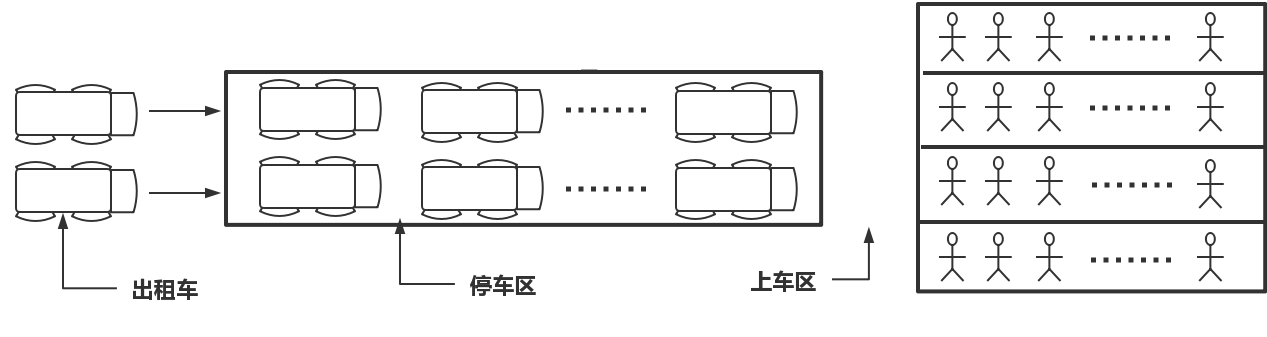
\includegraphics[width=.9\textwidth]{modle3}
	\caption{并行车道示意图}
	\label{fig:circuit-diagram}
\end{figure}
\newpage
机场出租车的运力需求因为航班航次,车队长度以及若干因素呈现出随机动态变化状态。若一味的增加服务设施即上客口,固然能解决乘客及出租车司机的排队现象,但存在极大导致资源浪费的可能,无法达到最大的经济效益。故本问的根本研究对象是出租车司机以及乘客的排队问题,合理安排上客口的数量,把双方的等待时间都尽量控制在一定的范围内从而在二者的等待时间内取得一定的平衡,在提高双方效率的同时避免过高的成本。

基于对飞机场上客区作业过程建立出租车上客区通行能力计算模型,优化出租车上客区的通行能力。并通过模型计算并统计出双车道情况下出租车上客口数量不同时的通行能力表,对双车道情况下出租车上客口的数量进行合理探讨。

将上客口都处于闲置状态的概率用$P_0$表示;将排队的平均乘客数量用$L_q$表示;正在上车的乘客数量记为$L_s$;每位乘客的平均等待时间为$W_q$;记司机的平均返回时间为$W_s$;乘客需排队等待的概率记为$P_w$。

\subsection{问题四的分析}
综合分析第三问所规划出的机场乘车设计图,可清晰地看出乘客可选择登上两条行车道上的任意一条。而对于返场重新载客的短途司机而言,其对接下来所接乘客要去往的目的地是未知的。而基于第二问对机场出租车载客数据进行的调查,出租车司机每次接客约有14.2$\%$的概率可接到长途乘客,且每次进入“蓄车池”排队的时长都不固定,主要分布在[0.5,3.0]小时的区间内。因此,这些返场短途出租车必须与第一次进入蓄车池或已经接过长途客人的返程出租车区分开来。而基于第三问所提出的两条“行车道”和优化出的乘客“上车点”,可调整短途出租车与其余排队出租车的顺序,以达到较为合理的“优先”。

\newpage
\section{模型的建立与求解}
\subsection{问题一模型的建立与求解}
\subsubsection{基于数据挖掘算法的决策树}
在现实中,出租车司机对于车流量与人流量的认知对出租车司机决策的影响甚至要大于数据统计实际结果,因此若要建立出租车司机的决策模型,需要充分调研出租车司机的经验认知,并根据其经验认知进行统计得出基于出租车司机角度等待时长的合理分段。根据假设将实际问题进行简化,依照属性划分标准对建立决策树所需要的不同属性进行划分,划分标称变量与有序变量,划分后子节点的不纯度度量是划分属性的最优度量,不纯度越低即纯度越高说明划分效果越好。

对不纯度度量进行计算,计算公式如下:
$$
\begin{array}{l}{\text { Entropy }(\mathrm{t})=-\sum_{\mathrm{j}=0 \mathrm{c}-1} \mathrm{p}(\mathrm{i} | \mathrm{t}) \log_{2}  \mathrm{p}(\mathrm{i} | \mathrm{t}), \text { Entropy }(\mathrm{t}) \in[0,1]} \\ {\text { Gini }(\mathrm{t})=1-\sum_{\mathrm{i}=0 \mathrm{c}-1}[\mathrm{p}(\mathrm{i} | \mathrm{t})]_{2}, \text { Gini }(\mathrm{t}) \in[0,0.5]} \\ {\text { ClassificationError }(\mathrm{t})=1-\operatorname{maxi}[\mathrm{p}(\mathrm{i} | \mathrm{t})]} \\ {\text { ClassificationError }(\mathrm{t}) \in[0,0.5]}\end{array}
$$

根据熵值,Gini值的以及分类误差的取值位置进行判断,如下图:
\begin{figure}[!h]
	\centering
	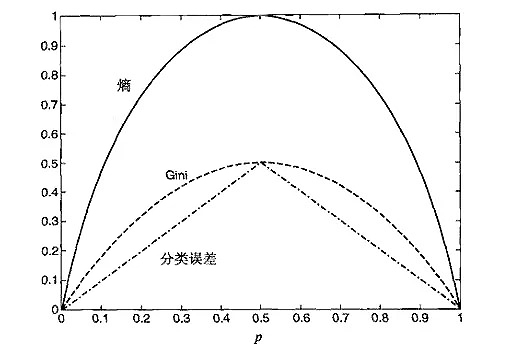
\includegraphics[width=.7\textwidth]{modle1}
	\caption{熵的参考值范围}
	\label{fig:circuit-diagram}
\end{figure}

取值越小时说明该属性越纯。

根据信息增益公式:
$$
\Delta=\mathrm{I}(\text { parent })-\sum_{\mathrm{j}=1}^{\mathrm{k}} \frac{\mathrm{N}\left(\mathrm{v}_{\mathrm{i}}\right)}{\mathrm{N}} \mathrm{I}\left(\mathrm{v}_{\mathrm{j}}\right)
$$

其中 I 为不纯度的度量,关于 N 的计算是划分后的个数加权。 
当I 为熵(Entropy)时,Delta 为信息增益,
由此我们可计算信息增益率:
$$
\text { GainRatio }=\Delta \text { infoSplitInfo }=\Delta \inf _{\mathrm{C}}-\sum_{\mathrm{C}}-\mathrm{i}_{\mathrm{i}=0 \mathrm{p}(\mathrm{i})} \log _{2} \mathrm{p}(\mathrm{i})
$$

然后根据假设将实际问题进行简化,并使用数据集进行挖掘算法计算,从而建立出租车司机的决策树模型,如下图:
\begin{figure}[!htbp]
	\centering
	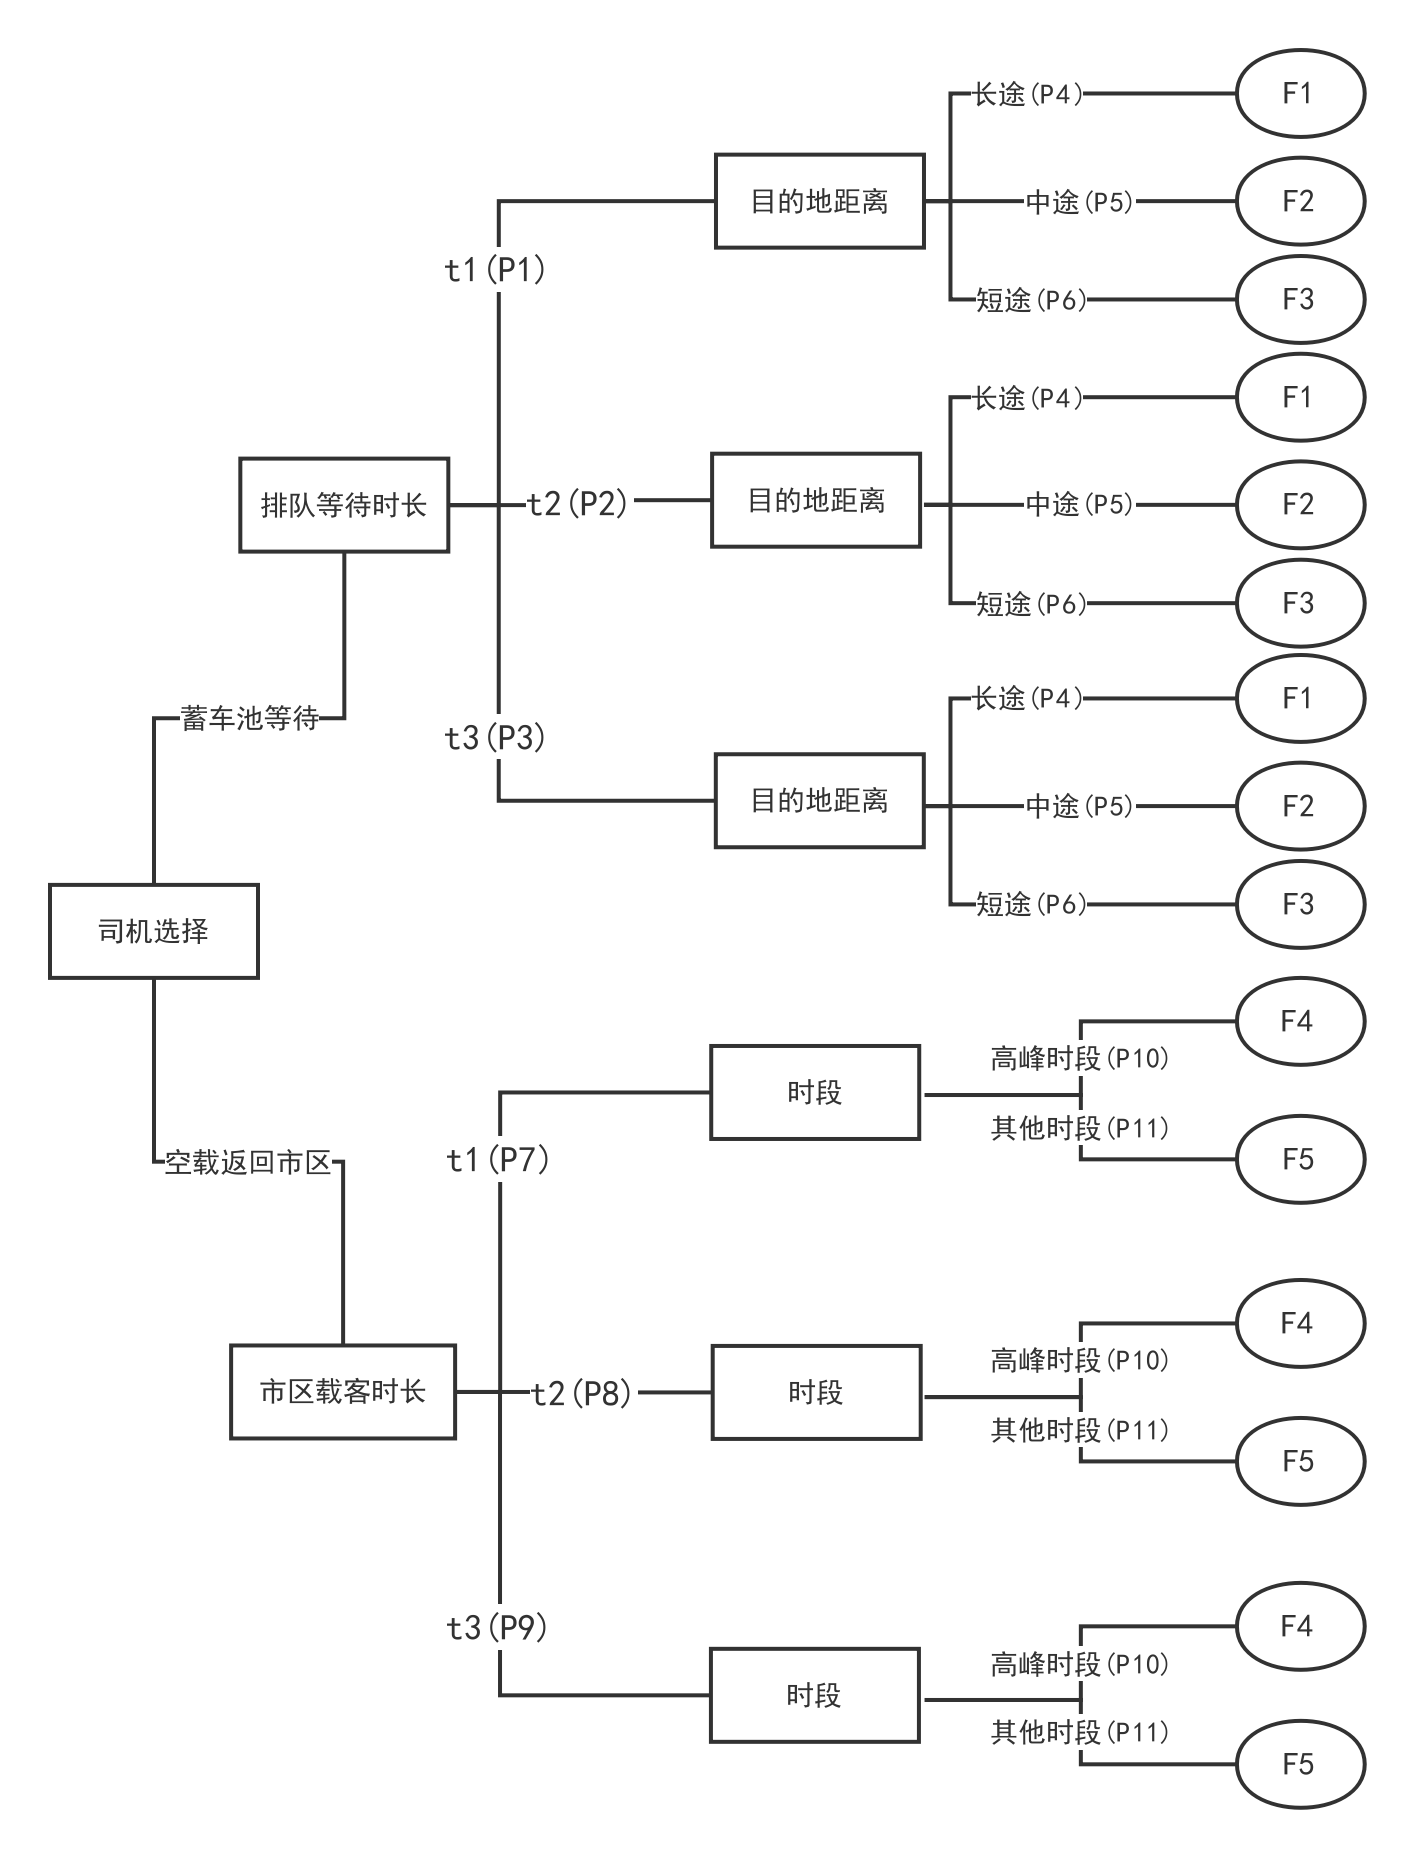
\includegraphics[width=.8\textwidth]{modle2}
	\caption{决策树}
	\label{fig:circuit-diagram}
\end{figure}

因为出租车司机可以观测到的某段时间内抵达的航班数量与“蓄车池”中已有车辆数会直接影响出租车司机对决定是否留在“蓄车池”中等待乘客这一问题的判断,并决定了出租车司机等客的时长,故将出租车司机选择在蓄车池等待时的排队时长分为$T_1,T_2,T_3$三类时间长度$\left(T_{1}<T_{2}<T_{3}\right)$,这三类时间长度都可根据出租车司机的个人经验被观测得到,且$T_1,T_2,T_3$所对应的概率分别设为$P_1,P_2,P_3$且$\Sigma_{1}^{i=3} P=1$。

由于出租车司机的损益值受到乘客目的地与机场实际距离的影响,故将乘客目的地与机场的距离分为长途,中途,短途三类,并将其损益值分别用$F_1,F_2,F_3$表示,且该损益值皆为观测值,可由数据统计得出该值。同时出租车司机接上长途乘客,中途乘客,短途乘客的的概率分别为P$_4,P_5,P_6$且$\sum_{3}^{i=6} P=1$。

用$E(X_1)$表示出租车司机选择在蓄车池等待状态下$T_1$时间段的预期收益,以$E(x_1)$, $E(x_2)$, $E(x_3)$分别表示接到长途乘客,中途乘客与短途乘客状态下出租车司机的预期收益。

即出租车司机在选择进入蓄车池等待这一状态下,于$T_1$时间段可以接到长途客人而获得的预期收益为
$$
\mathrm{E}\left(x_{1}\right)=F_{1} * P_{4} ; \quad(1)
$$

同理,出租车司机在选择进入蓄车池状态下于$T_1$时间段可以接到中途客人而获得的预期收益为
$$
\mathrm{E}\left(x_{2}\right)=F_{2} * P_{5} ; \quad(2)
$$

于$T_1$时间段可以接到短途客人而获得的预期收益为
$$
\mathrm{E}\left(x_{3}\right)=F_{3} * P_{6}; \quad(3)
$$

由公式(1),(2),(3)可得出租车司机在$T_1$时间段可获得的平均预期收益公式为
$$
\begin{array}{l}{\mathrm{E}\left(X_{1}\right)=\left(\mathrm{E}\left(x_{1}\right)+\mathrm{E}\left(x_{2}\right)+\mathrm{E}\left(x_{3}\right)\right) * P_{1}} \\ {=\left(F_{1} * P_{4}+F_{2} * P_{5}+F_{3} * P_{6}\right) * P_{1}} \quad(4)\end{array}
$$

以$E(X_2)$表示出租车司机选择在蓄车池等待状态下$T_2$时间段的预期收益,故:
$$
\begin{array}{l}{\mathrm{E}\left(X_{2}\right)=\left(\mathrm{E}\left(x_{1}\right)+\mathrm{E}\left(x_{2}\right)+\mathrm{E}\left(x_{3}\right)\right) * P_{2}} \\ {=\left(F_{1} * P_{4}+F_{2} * P_{5}+F_{3} * P_{6}\right) * P_{2}} \quad(5)\end{array}
$$

以$E(X_3)$表示出租车司机选择在蓄车池等待状态下$T_3$时间段的预期收益,故:
$$
\begin{array}{l}{\mathrm{E}\left(X_{3}\right)=\left(\mathrm{E}\left(x_{1}\right)+\mathrm{E}\left(x_{2}\right)+\mathrm{E}\left(x_{3}\right)\right) * P_{3} } \\ {=\left(F_{1} * P_{4}+F_{2} * P_{5}+F_{3} * P_{6}\right) * P_{3}} \quad(6)\end{array}
$$

在出租车司机选择返回市区的状态下且不考虑油料损失时,存在出租车司机面临$T_1$时间段的等待时长时选择返回市区,面临$T_2$时间段的等待时长时选择返回市区以及面临$T_3$时间段的等待时长时选择返回市区的三种情况。此时,将司机面临$T_1,T_2,T_3$三类等待时间时选择返回市区并且可以避免空载的概率分别用$P_7,P_8,P_9$来表示。

同时,以$P(10),P(11)$表示出租车司机在返程时面临高峰时段和其他时段的两种概率$\left(\sum_{10}^{i=11} P=1\right)$,因为已在模型假设中排除节假日,天气等因素的影响,所以城市的高峰时段分布服从U分布并具有可预测的不变性规律。所以高峰时段及其他时段每天出现的概率相等,分别获得的损益也相等,并用$F_4,F_5$分别表示出租司机在高峰时段与其他时段的损益值。

分别用$E(Y_1)$,$E(Y_2)$,$E(Y_3)$表示出租车司机在需面临蓄车池$T_1,T_2,T_3$三类时间长度的等待状态下选择返回市区的预期收益,并且以$E(y_1), E(y_2), E(y_3)$分别表示接到长途乘客,中途乘客与短途乘客状态下出租车司机的预期收益。

故
$$\mathrm{E}\left(y_{1}\right)=F_{4} * P_{10}+F_{5} * P_{11}$$

且
$$\mathrm{E}\left(y_{1}\right)=\mathrm{E}\left(y_{2}\right)=\mathrm{E}\left(y_{3}\right)$$

所以
$$\mathrm{E}\left(y_{1}\right)=\mathrm{E}\left(y_{2}\right)=\mathrm{E}\left(y_{3}\right)=F_{4} * P_{10}+F_{5} * P_{11} \quad(7)$$

由(7)可知出租车司机面临需在蓄车池等待$T_1$时间长度的状态下选择返回市区的预期收益为$$\mathrm{E}\left(Y_{1}\right)=\mathrm{E}\left(y_{1}\right) * P_{7}=\left(F_{4} * P_{10}+F_{5} * P_{11}\right) * P_{7} ; \quad(8)$$

出租车司机面临需在蓄车池等待$T_2$时间长度的状态下选择返回市区的预期收益为
$$\mathrm{E}\left(Y_{2}\right)=\mathrm{E}\left(y_{2}\right) * P_{8}=\left(F_{4} * P_{10}+F_{5} * P_{11}\right) * P_{8} \quad(9)$$

出租车司机面临需在蓄车池等待$T_3$时间长度的状态下选择返回市区的预期收益为
$$\mathrm{E}\left(Y_{3}\right)=\mathrm{E}\left(y_{3}\right) * P_{9}=\left(F_{4} * P_{10}+F_{5} * P_{11}\right) * P_{9} \quad(10)$$

通过出租车司机选择在蓄车池等待状态下$T_1$时间段的预期收益$E(X_1)$与出租车司机面临需在蓄车池等待$T_1$时间长度的状态下选择返回市区的预期收益$E(Y_1)$;出租车司机选择在蓄车池等待状态下$T_2$时间段的预期收益$E(X_2)$与出租车司机面临需在蓄车池等待$T_2$时间长度的状态下选择返回市区的预期收益$E(Y_2)$;出租车司机选择在蓄车池等待状态下$T_3$时间段的预期收益$E(X_3)$与出租车司机面临需在蓄车池等待$T_3$时间长度的状态下选择返回市区的预期收益$E(Y_3)$三组数据的比较得出不同状态下最适宜于出租车司机的选择决策。选择策略表示如下表:
\begin{comment}
\section{绘制普通三线表格}
表格应具有三线表格式,因此常用 booktabs宏包,其标准格式如\cref{tab:001}~所示。
\end{comment}
\begin{table}[!htbp]
	\caption{选择策略表}\label{tab:001} \centering
	\begin{tabular}{ccccc}
		\toprule[1.5pt]
		  \qquad & $\mathrm{E}\left(X_{1}\right) \geq \mathrm{E}\left(Y_{1}\right)$ & $\mathrm{E}\left(X_{2}\right) \geq \mathrm{E}\left(Y_{2}\right)$ & $\mathrm{E}\left(X_{3}\right) \geq \mathrm{E}\left(Y_{3}\right)$\\
		\midrule[1pt]
		是 & 等待 & 等待 & 等待\\
		否 & 直接返回 & 直接返回 & 直接返回\\
		\bottomrule[1.5pt]
	\end{tabular}
\end{table}

\newpage
若$E(X_1)≥E(Y_1)$,即当出租车司机根据车流量与人流量状况并通过经验判断出留在“蓄车池”中等乘客需花费$T_1$时间时,通过决策树计算得出的出租车司机的预期收益确实大于选择直接返回市区的预期收益,则出租车司机应在此时选择进入蓄车池等待乘客,若$E(X_1)≤E(Y_1)$,则出租车司机应选择不进入蓄车池直接返回市区。同理,当出租车司机根据现场车流量及即将到达航班次判断出若进入蓄车池等待时间应为$T_2$,$T_3$段时间长度时,若$E(X_2)≥E(Y_2)$与$E(X_3)≥E(Y_3)$,出租车司机也应在此两种情况下分别选择进入蓄车池等待乘客,反之则应选择直接返回市区。

\subsection{问题二模型的建立与求解}
\subsubsection{损益值的计算}
筛选发车地点位于北京市首都国际机场内的出租车的行车轨迹数据。根据高德地图测算出北京市各区的中心距首都国际机场的距离,并可由高德地图软件自动生成乘坐出租车由首都国际机场出发,目的地为各区中心的乘客乘车费用,即出租车司机的实际收益。对不同的地区按距离与乘车费用进行分类,将北京市十六个区县按其距离首都国际机场的距离分为远程,中程,进程三类,其各自费用表如下:

远距乘客费用比例表为:
\begin{table}[!htbp]
	\caption{远距离乘车费用比例表}\label{tab:001} \centering
	\begin{tabular}{ccccc}
		\toprule[2pt]
		区,县 & 司机收益(元) & 所占比例\\
		\midrule[1pt]
		昌平区 & 170 & 29$\%$\\
		平谷区 & 158 & 17$\%$\\
		密云区 & 158 & 23$\%$\\
		延庆区 & 290 & 11$\%$\\
		房山区 & 180 & 20$\%$\\
		\bottomrule[1.5pt]
	\end{tabular}
\end{table}

所以,$F_{1}=170 \times 29 \%+158 \times 17 \%+158 \times 23 \%+290 \times 11 \%+180 \times 20 \%=$
180.40$({\text{元}})$\\

中距乘客费用比例表为:

\begin{table}[!htbp]
	\caption{中距离乘车费用比例表}\label{tab:001} \centering
	\begin{tabular}{ccccc}
		\toprule[2pt]
		区,县 & 司机收益(元) & 所占比例\\
		\midrule[1pt]
		怀柔区 & 105 & 10$\%$\\
		门头沟区 & 142 & 21$\%$\\
		丰台区 & 122 & 24$\%$\\
		大兴区 & 136 & 16$\%$\\
		石景山区 & 131 & 10$\%$\\
		海淀区 & 104 & 19$\%$\\
		\bottomrule[1.5pt]
	\end{tabular}
\end{table}

所以,$F_{2}=105 \times 10 \%+142 \times 21 \%+122 \times 24 \%+136 \times 16 \%+131 \times 10 \%+$
$104 \times 19 \% \approx 124.22({\text{元}})$

近距乘客费用比例表为:

\begin{table}[!htbp]
	\caption{近距离乘车费用比例表}\label{tab:001} \centering
	\begin{tabular}{ccccc}
		\toprule[2pt]
		区,县 & 司机收益(元) & 所占比例\\
		\midrule[1pt]
		通州区 & 30 & 10$\%$\\
		顺义区 & 45 & 21$\%$\\
		东城区 & 70 & 24$\%$\\
		西城区 & 90 & 16$\%$\\
		朝阳区 & 69 & 10$\%$\\
		崇文区 & 80 & 19$\%$\\
		宣武区 & 92 & 10$\%$\\
		\bottomrule[1.5pt]
	\end{tabular}
\end{table}

所以,$F_{3}=30 \times 13 \%+45 \times 11 \%+70 \times 17 \%+90 \times 15 \%+69 \times 21 \%+$
$80 \times 13 \%+92 \times 10 \%=68.34({\text{元}}) $;

在现实中,出租车司机对于车流量与人流量的认知对出租车司机决策的影响甚至要大于数据统计实际结果,因此若要建立出租车司机的决策模型,需要充分调研出租车司机的经验认知,并根据其经验认知进行统计得出基于出租车司机角度等待时长的合理分段,如下表:

\begin{table}[!htbp]
	\caption{司机蓄车池等待时间分布}\label{tab:001} \centering
	\begin{tabular}{ccccc}
		\toprule[2pt]
		时间段分布& 根据提供者数量确定的权重\\
		\midrule[1pt]
		$0^{\sim} 30$ & 15$\%$\\
		$31^{\sim} 60$ & 43$\%$\\
		$61^{\sim} 120$ & 34$\%$\\
		120分钟及以上 & 8$\%$\\
		\bottomrule[1.5pt]
	\end{tabular}
\end{table}

\subsubsection{概率值的测算}
由于已知出租车司机航班航次信息并具有丰富经验,故其可根据实际车流量较为准确的预估出若选择进入蓄车池将需要等待的时间。由于出租车司机的经验具有普适性并可实地调研,考虑到出租车司机的个人经验在其决策中占有较大的影响,故经过作者实地调研后总结出150位出租车司机的经验进行统计分析。根据司机提供的经验统计分析得出$T_1$,$T_2$,$T_3$的合理时间长度与乘客目的地距机场距离远,中,近的三类概率,即$P_1$,$P_2$,$P_3$的概率。
\begin{table}[!htbp]
	\caption{接到远程乘客的概率$P_1$的分布}\label{tab:001} \centering
	\begin{tabular}{ccccc}
		\toprule[1.5pt]
		司机接到远程乘客的比例& 提供者数量权重\\
		\midrule[1pt]
		$\frac{1}{5}$ & 48$\%$\\
		$\frac{1}{8}$ & 16$\%$\\
		$\frac{1}{10}$ & 30$\%$\\
		$\frac{1}{15}$ & 12$\%$\\
		\bottomrule[1.5pt]
	\end{tabular}
\end{table}

根据远程乘客所占比例以及提供者数量的权重可以计算出出租车司机选择进入“蓄车池”后接到远程乘客的概率$P_1$为
$$
P_{1}=\frac{1}{5} * 42 \%+\frac{1}{8} * 16 \%+\frac{1}{10} * 30 \%+\frac{1}{15} 12 \% \approx 14.2 \%
$$

\begin{table}[!htbp]
	\caption{接到中程乘客的概率$P_2$的分布}\label{tab:001} \centering
	\begin{tabular}{ccccc}
		\toprule[1.5pt]
		司机接到近程乘客的比例& 提供者数量权重\\
		\midrule[1pt]
		$\frac{1}{2}$ & 26$\%$\\
		$\frac{1}{3}$ & 24$\%$\\
		$\frac{1}{4}$ & 30$\%$\\
		$\frac{1}{5}$ & 22$\%$\\
		\bottomrule[1.5pt]
	\end{tabular}
\end{table}

根据中程乘客所占比例以及提供者数量的权重可以计算出出租车司机选择进入“蓄车池”后接到中程乘客的概率$P_2$为
$$
P_{2}=\frac{1}{2} * 26 \%+\frac{1}{3} * 24 \%+\frac{1}{4} * 30 \%+\frac{1}{5} 22 \% \approx 32.9 \%
$$

\begin{table}[!htbp]
	\caption{接到近程乘客的概率$P_3$的分布}\label{tab:001} \centering
	\begin{tabular}{ccccc}
		\toprule[1.5pt]
		司机接到近程乘客的比例& 提供者数量权重\\
		\midrule[1pt]
		$\frac{1}{3}$ & 41$\%$\\
		$\frac{1}{2}$ & 30$\%$\\
		$\frac{2}{3}$ & 16$\%$\\
		$\frac{3}{4}$ & 13$\%$\\
		\bottomrule[1.5pt]
	\end{tabular}
\end{table}

根据近程乘客所占比例以及提供者数量的权重可以计算出出租车司机选择进入“蓄车池”后接到近程乘客的概率$P_3$为
$$
P_{3}=\frac{1}{3} * 41 \%+\frac{1}{2} * 30 \%+\frac{2}{3} * 16 \%+\frac{3}{4} 13 \% \approx 49.1 \%
$$

并通过数据查询得到$P_{4}=25 \% ; P_{5}=75 \%$

\subsubsection{模型求解}
将实际数据代入第一问决策树模型求解结果,得;

$$
\mathrm{E}\left(X_{1}\right)=\left(\mathrm{E}\left(x_{1}\right)+\mathrm{E}\left(x_{2}\right)+\mathrm{E}\left(x_{3}\right)\right) * P_{1}=36
$$
$$
\begin{array}{l}{\mathrm{E}\left(X_{2}\right)=\left(\mathrm{E}\left(x_{1}\right)+\mathrm{E}\left(x_{2}\right)+\mathrm{E}\left(x_{3}\right)\right) * P_{2}} \\ {\quad=\left(F_{1} * P_{4}+F_{2} * P_{5}+F_{3} * P_{6}\right) * P_{3}}=39\end{array}
$$
$$
\begin{array}{l}{\mathrm{E}\left(X_{3}\right)=\left(\mathrm{E}\left(x_{1}\right)+\mathrm{E}\left(x_{2}\right)+\mathrm{E}\left(x_{3}\right)\right) * P_{3}} \\ {=\left(F_{1} * P_{4}+F_{2} * P_{5}+F_{3} * P_{6}\right) * P_{3}}=41\end{array}
$$

\subsubsection{模型的合理性分析}
\textbf{1、Gini值验证样本选取的合理性}

首先对数据进行排序并按照离散点的取值进行计算,计算GINI和熵趋向于有大量不同值的属性。

记Ni为第i个子节点的数据个数,Ginii即第i个子节点的Gini指标,此时权重为子节点的数据量占比。

根据公式
$$
\operatorname{Gini}(D)=1-\sum_{i=1}^{m} p_{i}^{2}=\sum_{i=1}^{m} p_{i}^{*}(1-p)
$$
计算得出各节点GINI值如下表:
\begin{table}[!htbp]
	\caption{各节点GINI值分布表}\label{tab:006} \centering
	\begin{tabular}{ccccc}
		\toprule[2pt]
		相应节点 & GINI值 & 相应节点 & GINI值\\
		\midrule[1pt]
		$T_{1}\left(P_{1}\right)$ & 0.420 & 长途 & 0.300\\
     	$T_{2}\left(P_{2}\right)$ & 0.400 & 中途 & 0.343\\
		$T_{3}\left(P_{3}\right)$ & 0.375 & 短途 & 0.375\\
		$T_{1}\left(P_{4}\right)$ & 0.343 & 高峰时段 & 0.400\\
		$T_{2}\left(P_{5}\right)$ & 0.417 & 其他时段 &0.420\\
		$T_{3}\left(P_{6}\right)$ & 0.400\\
		\bottomrule[1.5pt]
	\end{tabular}
\end{table}

因为上述Gini值皆小于0.5且数值都较小,所以选取样本的纯净度较高,模型较为合理。

\textbf{2、决策树分类模型的评分函数}

$(1)$预测准确率
模型总体准确率计算公式为:
$$
\text{全体准确率}=\frac{\text{预测正确的纪录数}}{\text{全部记录数}} \times 100 \%
$$

计算得出全体准确率=69.276$\%$

模型相对预测准确率计算公式为:
$$
\text{相对预测准确率}=\frac{{\text{该类预测准确率}}-{\text{该类实际样本数}}/{\text{训练集数}}}{{\text{该类实际样本数}}/{\text{训练集数}}} \times 100 \%
$$
由此可计算得各项分类的相对预测准确率,如下表:
\begin{table}[!h]
	\caption{各项分类相对预测准确率分布表}\label{tab:007} \centering
	\begin{tabular}{ccccc}
		\toprule[2pt]
		乘客搭车目的地路途长短分类& 相对预测准确率 & 时长分类 & 相对预测准确率\\
		\midrule[1pt]
		长途 & 76.712$\%$ & 高峰时段 & 82.314$\%$\\
		中途 & 61.643$\%$ & 其他时段 & 54.223$\%$\\
		短途 & 48.661$\%$\\
		\bottomrule[1.5pt]
	\end{tabular}
\end{table}

因为全体准确率与相对预测准确率都较高,故模型合理性较高。

$(2)$过度拟合阈值

通常情况下取50$\%$的阈值以检验决策树的过度拟合的可能性,
$$
\text{叶子数为1的分支数}=\frac{\text{叶子数为1的分支数}}{\text{总分支数}} \times 100 \%
$$

当叶子数为1的分支数$>50$$\%$时,存在过度拟合的情况。

由公式计算得叶子数为1的分支数为0,所以本模型不存在过度拟合状态,模型设立较为合理。

$(3)$健壮性(L)评判
$$
\mathrm{L}=L_{1}+L_{2}
$$

且
$$
L_{1}=1-({\text{叶子节点为1的分支数}} / {\text{总分支数}}) \times 100 \% ; 
L_{2}=\left(\frac{{\text{叶子数}}}{{\text{节点数}}}\right) \times 100 \%;
$$

因为$L_{1}=1, \quad L_{2}=62.5 \%$,所以$\mathrm{L}=162.5 \%>1$。

说明模型设立的决策树比较健壮,模型合理性较高。\upcite{__2005}
\newpage
\subsection{问题三模型的建立与求解}
\subsubsection{出租车上客区通行能力配置与优化模型}
\textbf{1、概率优化模型的建立}

出租车上客区作业过程示意图如下:
\begin{figure}[!htbp]
	\centering
	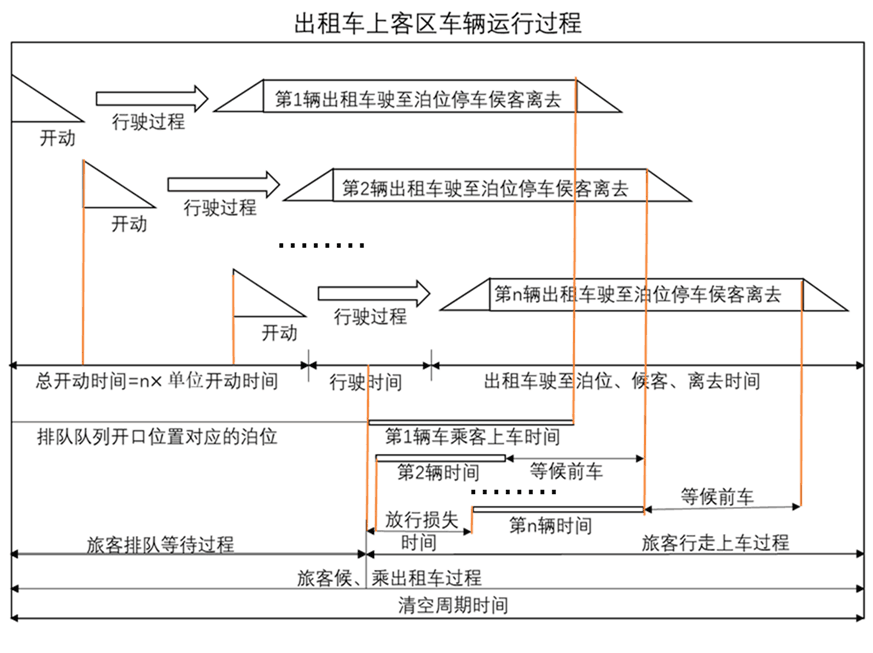
\includegraphics[width=.9\textwidth]{modle4}
	\caption{出租车上客区作业过程示意图}
	\label{fig:circuit-diagram}
\end{figure}

假设两列车道均为单行道,建立出租车上客区通行能力计算模型为:
$$
\max Q=N_{\text {泊位}} \times P_{\mathrm{L}} \times 3600 / T_{\text {空出}}
$$

与模型作用机理相关的各项因素分别用公示表示为:

(1)上客口数量为:
$$
N_{\text{泊位}}=n_{\text{车道数}} \times n_{\text{单道泊位数}}
$$

(2)上客区空出周期时间$T_{\text{空出}}$ :
$$
\begin{array}{l}{T_{\text{空出}}=n_{\text{单道泊位数}} t_{\text{开动}}+t_{\text{行驶}}+t_{\text{停车}}+t_{\text{候客}}+t_{\text{开动}}=} \\ {\quad\left\langle n_{\text{单道泊位数}}+1\right) t_{\text{开动}}+t_{\text{行驶}}+t_{\text{停车}}+t_{\text{候客}}}\end{array}
$$

(3)出租车司机在蓄车池中等待的时间
$$
t_{\text{停车}}=i \times t_{\text{开动}}+t_{\text{行驶}}+t_{\text{停车}}
$$

(4)出租车司机在进入上客口前等待的时间:
$$
t_{\text{离去}}=i \times t_{\text{开动}}+t_{\text{行驶}}+t_{\text{停车}}+t_{\text{候客}}
$$

(5)出租车司机从蓄车池行至上客口所需时间:
$$
t_{\text{行驶}}=n_{\text{单道泊位数}} \times L / v_{\text{车}}
$$

(6)出租车司机等待乘客的时间为:
$$
t_{i \text{候客}}=\max \left(t_{i-1 \text{离去}}+t_{\text{开动}}, t_{i \text{乘客}}\right)
$$

(7)乘客从进入等待区直到下车所耗费的时间:
$$
t_{i {\text{乘客}}}=f_{\text{放}}+t_{i {\text{放行}}}+t_{i {\text{行走}}}+t_{\text{放置行李}}+t_{\text{登车}}
$$

(8)乘客从等待区行至上客口所需时间:
$$
t_{i \text{放行}}=n_{\text{车道数}} \times i \times P_{L} \times S
$$

(9)为保证乘客安全,出租车司机应该在乘客走到上客口前将车停稳,故针对与安全约束条件为:
$$
t_{i \text{停车}} \leq f_{\text{放}}+t_{i \text{放行}}+t_{i \text{行走}}
$$

且
$$
f_{\text{放}} \geqslant t_{{W}_{\text{开口}} \text{停车}}
$$

最终得出出租车在上客口的最大通行能力。

\textbf{2、优化模型的求解}

调研结果显示,出租车上客口的各类基本指标的参数值如下表:
\begin{table}[!htbp]
	\caption{出租车基本指标参数表}\label{tab:008} \centering
	\begin{tabular}{ccccc}
		\toprule[2pt]
		基本参数 & 取值 & 基本参数 & 取值\\
		\midrule[1pt]
		出租车平均车速$v_{\text{车}}/(m/s)$ & 3	& 泊位长度$L/m$ & 5\\
		车辆平均开动时间$t_{\text{开动}}/s$ & 3 & 乘客登车消耗时间$t_{\text{登车}}/s$ & 2\\
	    车辆平均停车时间$t_{\text{停车}}/s$ & 3 &
	    车均载客人数$P_L/({\text{人}}/{\text{车}})$ & 1.5\\
		乘客平均行速度$v_{\text{人}}/(m/s)$ & 1.5 & 开口放行单位乘客平均消耗时间$S/s$ & 1\\
		\bottomrule[1.5pt]
	\end{tabular}
\end{table}
\newpage
通过上述参数计算双车道出租车上客通行能力,得到双车道下的出租车上客口通行能力分析图如下:
\begin{figure}[!htbp]
	\centering
	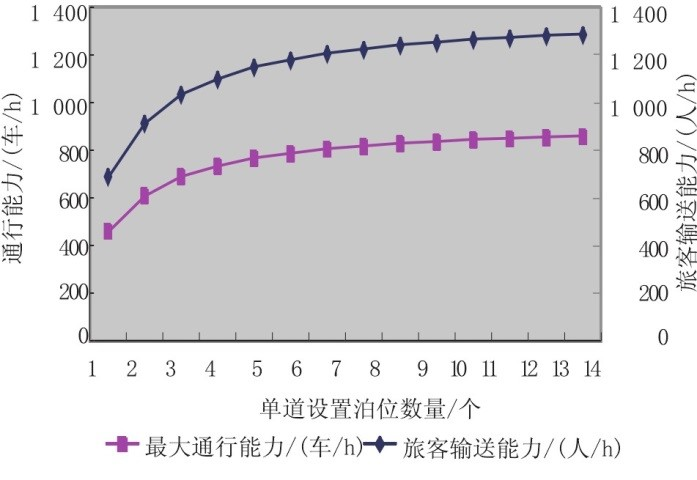
\includegraphics[width=.8\textwidth]{modle5}
	\caption{双车道出租车通行能力分析图}
	\label{fig:circuit-diagram}
\end{figure}

由图可知初始时通行能力会随上客口的增加递增,但是随着上客口数量的增加,通行能力边际增长率逐渐下降,通过计算得到双车道出租车上客区的通过能力表:

\begin{table}[!htbp]
	\caption{双车道出租车上客区的通过能力表}\label{tab:008} \centering
	\begin{tabular}{ccccc}
		\toprule[2pt]
		单道泊位数/个 & 空出周期时间/s & 最大通行能力/(车/h) & 最大通行能力/(车/h)\\
		\midrule[1pt]
		1 & 15.7 & 460 & 689\\
    	2 & 23.7 & 608 & 913\\ 
	    3 & 31.3 & 689 & 1034\\
	    4 & 39.3 & 732 & 1098\\
	    5 & 47.0 & 766 & 1149\\
	    6 & 55.0 & 785 & 1178\\
	    7 & 62.7 & 804 & 1206\\
	    8 & 70.7 & 815 & 1223\\
	    9 & 78.3 & 827 & 1241\\
	    10 & 86.3 & 834 & 1251\\
	    11 & 94.0 & 843 & 1264\\
    	12 & 102.0 & 847 & 1271\\
	    13 & 109.7 & 853 & 1280\\
	    14 & 117.7 & 857 & 1285\\
		\bottomrule[1.5pt]
	\end{tabular}
\end{table}
\newpage
由表可知,当车道为双车道时,上客口数量应控制在$8^{\sim} 11$个,此时双方的效益基本达到了平衡,在一定程度上实现了最优。\upcite{__2017}


\subsubsection{出租车载客运输模型}
\upcite{__2018}
设机场内排队等候出租车的乘客每分钟的数量变化为:
$$
p_{\text{乘客每分钟变化数目}}=\sum p_{\text{乘客进入数}}-\sum p_{\text{乘客离开数}}
$$

因此机场内等候出租车的乘客数目为:
$$
p_{\text{乘客等候总数}}=p_{\text{乘客原本等候数}}+p_{\text{乘客每分钟变化数目}}
$$


同样,机场内每分钟在“蓄车池”中排队的出租车数变化为:
$$
p_{\text{出租车每分钟变化数目}}=\sum p_{\text{出租车入场数}}-\sum p_{\text{出租车离开数}}
$$

因此首都机场内排队的出租车数为:
$$
p_{\text{出租车等候总数}}=p_{\text{出租车原本等候数}}+p_{\text{出租车每分钟变化数目}}
$$

根据调查所得出每次出租车司机接到短途旅客的概率为49.1$\%$,因此可根据第三问中所设计的乘客“上车点”,在旅客下飞机的过程中,通过询问旅客目的地并将这些信息导入智能调度系统。经过人工智能的分析,将短途旅客分配到同一乘车点,同时,在此行车道排队的短途出租车司机也可在送完一组乘客后再次返场,进入同一乘车到继续等候。但这种方案存在一种弊端,即大约一半的短途出租车都一直在送短途乘客,其在短途往返中所要付出的成本与其获得的收益是无法与长途出租车司机达到基本平衡的。另外,长时间的短途往返与“蓄车池”等待必然会导致司机的负面情绪,因此需要一个更完备的设计方案。

\subsection{问题四模型的建立与求解}
\subsubsection{多通道等待制排队模型}
根据第三问所设计的两条“行车道”,假设排队等候乘客服从Poisson分布,平均每分钟$P_{\text{乘客每分钟变化数目}}$辆出租车排队等候搭载乘客,乘客等候的时间服从负指数分布,每个乘客乘车通道每分钟变化的人数为$P_{\text{乘客每分钟变化数目}}$,建立多通道等待制排队模型。

其中,t为任意某分钟,设:

$$
\mathrm{X}(\mathrm{t})=P_{\text{乘客每分钟变化数目}}
$$
$$
\mathrm{Y}(\mathrm{t})=P_{\text{乘客每分钟变化数目}}
$$

则出租车排队的平均队长为
$$
\mathrm{L}=\sum_{n=0}^{\infty} n P_{n}=\frac{\rho}{1-\rho}=\frac{\lambda}{1-\lambda}
$$

出租车的平均等待时间为:
$$
\omega=\frac{1}{\mu-\lambda}
$$

而对于短途司机从搭载第i车乘客到返场搭载第(i+1)车乘客的时间间隔τ服从参数为$\omega$的指数分布:
$$
P_{r}\left\{\tau_{n} \leq t\right\}=\left\{\begin{array}{ll}{1-e^{-\lambda t}} & {t \geq 0} \\ {0} & {t<0}\end{array}\right.
$$

通过以上模型可结合数据进行求解。

假设某短途返程出租车M排在当前出租车队列的队尾,即其前面共有$\frac{\lambda}{1-\lambda}-1$辆出租车。

由于其返程时间大于1小时的概率为$1-e^{-60 \lambda}$,假设这一阶段司机的有效行驶时间为50分钟,且认为出租车司机恒以60km/h的速度行驶,即可计算这段时间内出租车司机的经营成本。同时也必须考虑司机在“蓄车池”中排队所带来的成本,将此成本与短程出租车司机搭载客人所带来的收益进行比较,若成本小于收益的70$\%$,则确定此时的队伍长度,将为短途出租车司机开设次长度的VIP绿色通道,以提高其收益。VIP绿色通道的设计方式如下图所示:

\begin{figure}[!h]
	\centering
	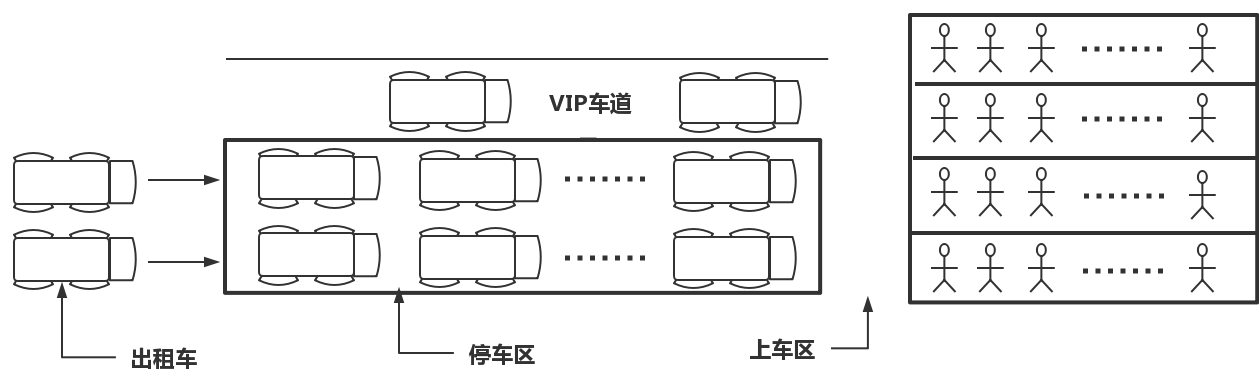
\includegraphics[width=.7\textwidth]{modle6}
	\caption{短途返程出租车VIP绿色通道示意图}
	\label{fig:circuit-diagram}
\end{figure}

\subsubsection{多服务台泊松到达,负指数服务时间,系统容量有限制的排队模型}
c为车站设置的上客口的数量\upcite{__2015};

模型中的到达率
$$
\lambda_{n}=\left\{\begin{array}{c}{\lambda, n=0,1, \ldots, K-1} \\ {0, n=K}\end{array}\right.
$$
$$
\mu_{n}=\left\{\begin{array}{l}{n \mu, 0 \leq n<a} \\ {a \mu, \varphi \leq n \leq K}\end{array}\right.
$$

使得$\rho=\frac{\lambda}{c \mu}$,且对任意$\mathbf{n} \geq \mathbf{K}$;

同时$\lambda_{n}=0, \mu_{n}=c \mu$

并且λ<μ,即到达率小于服务率,排队长度增加受到限制,

则有(1)
$$
P_{0}=\left\{\begin{array}{ll}{\left[\sum_{n=0}^{c-1} \frac{(c \rho)^{n}}{n !}+\frac{c^{c}}{c !} \frac{\left(\rho^{c}-\rho^{K+1}\right)}{1-\rho}\right]^{-1},} & {\rho \neq 1} \\ {\left[\sum_{n=0}^{c-1} \frac{(c \rho)^{n}}{n !}+\frac{(c \rho)^{c}}{c !}(K-c+1)\right]^{-1},} & {\rho=1}\end{array}\right. \quad(11)
$$

(2)单个上客口恰好有n个乘客的概率
$$
P_{n}=\left\{\begin{array}{ll}{\frac{(c \rho)^{n}}{n !} P_{0},} & {n=1,2, \cdots, c-1} \\ {\frac{c^{c}}{c !} \rho^{n} P_{0},} & {n=c, c+1, \cdots, K}\end{array}\right. \quad(12)
$$

(3)正在排队等待的平均顾客数
$$
\begin{array}{c}{L_{\mathrm{q}}=\sum_{n=c}^{K}(n-c) P_{n}} \\ \\ {L_{\mathrm{q}}=\left\{\begin{array}{ll}{\frac{P_{0}(c \rho)^{\mathrm{c}}}{c !(1-\rho)^{2}}\left[1-\rho^{K-c+1}-(1-\rho)(K-c+1) \rho^{K-c}\right],} & {\rho \neq 1} \\ {\frac{P_{0}(c \rho)^{\mathrm{c}}}{2 c !}(K-c)(K-c+1),} & {\rho=1}\end{array}\right.}\end{array} \quad(13)
$$

(4)上客口的平均顾客数
$$
L_{\mathrm{s}}=L_{\mathrm{q}}+c \rho\left(1-P_{K}\right) \quad(14)
$$

(5)有效到达率


当一批发车数小于K时,乘客进入上客口的概率为λ;当一批发车等于K时,允许顾客进入上客口的概率为0;即在单位时间里进入上客口的平均顾客数便是有效到达率,为
$$
\lambda_{0}=\lambda\left(1-P_{K}\right)+0 \cdot P_{K}=\lambda\left(1-P_{K}\right) \quad(15)
$$

(6)乘客花在排队上的平均时间为
$$
W_{q}=\frac{L_{q}}{\lambda\left(1-P_{K}\right)}=\frac{L_{q}}{\lambda_{e}}  \quad(16)
$$

(7)乘客在上客口的平均逗留时间为
$$
W_{s}=\frac{L_{s}}{\lambda\left(1-P_{K}\right)}=\frac{L_{s}}{\lambda_{c}}  \quad(17)
$$

\subsubsection{排队模型的求解}
由于在第三问中已根据模型求解出双车道时,上客口数量应控制在8~11个,此时双方的效益基本达到了平衡,在一定程度上实现了最优。故此时应选取8~11个上客口的均值作为本问中上客口数量的实际取值,即9.5个。

运用“管理运筹学软件”生成计算结果:
\begin{table}[!htbp]
	\caption{双车道出租车上客区的通过能力表}\label{tab:009} \centering
	\begin{tabular}{ccccc}
		\toprule[2pt]
		参数 & $W_q$ & $W_s$ & $\lambda$ & $\mu$\\
		\midrule[1pt]
		实际值 & 25.8(min) & 3.4(min) & 0.6(人/min) & 0.6(人/min)\\
		\bottomrule[1.5pt]
	\end{tabular}
\end{table}
故通过出租车排队管理系统实现对出租车车牌的自动识别以计算其往返时间与行车里程,并由系统自动收发进出号码牌作为出租车是否可取得优先权的根据,往返时间在25.8min以下的车辆给予优先权,并为其单独安排一条行车通道通过优先权缩短短途司机等待时间,提高短途司机载客频率以补偿短途司机的权益。
\newpage

\bibliography{ref}

\newpage
%附录
\begin{appendices}

\section{通过经纬度求距离--java源程序}

\begin{lstlisting}[language=java]
public class Location{
private static double EARTH_RADIUS = 6378.137;

private static double rad(double d) {
return d * Math.PI / 180.0;
}
/**
* 通过经纬度获取距离(单位:米)
* @param lat1
* @param lng1
* @param lat2
* @param lng2
* @return 距离
*/
public static double getDistance(double lat1, double lng1, double lat2, double lng2) {
double radLat1 = rad(lat1);
double radLat2 = rad(lat2);
double a = radLat1 - radLat2;
double b = rad(lng1) - rad(lng2);
double s = 2 * Math.asin(Math.sqrt(
Math.pow(Math.sin(a / 2), 2) + Math.cos(radLat1) * Math.cos(radLat2) * Math.pow(Math.sin(b / 2), 2)));
s = s * EARTH_RADIUS;
s = Math.round(s * 10000d) / 10000d;
s = s * 1000;
return s;
}
}
public class main {
public static void main(String[] args) {
LocationUtils a=new LocationUtils();
double distance = a.getDistance(40.042,116.562,40.118,116.626);//
System.out.println("距离" + distance / 1000 + "公里");
}
}
\end{lstlisting}
\newpage

\section{处理出租车txt数据--python源程序}

\begin{lstlisting}[language=python]
# 批量读取北京市2008年2月的出租车数据,转换成csv格式。
import os
import csv
def eachFile(filepath):
pathDir = os.listdir(filepath)
pathtxt_list = []
for allDir in pathDir:
child = os.path.join('%s%s' % (filepath, allDir))
pathtxt_list.append(child.encode('utf-8').decode('gbk'))
return pathtxt_list

def readFile(filename):
fopen = open(filename, 'r')
f_list = []
for eachLine in fopen:
f_list.append(eachLine.strip('\n'))
fopen.close()
return f_list

def csvsave(taxi_list_1):
with open('taxi.csv', 'wb') as myFile:
myWriter = csv.writer(myFile)
myWriter.writerow(['taxi_id', 'date_time', 'lon', 'lat'])
myWriter.writerows(taxi_list_1)
# 主程序
pathtxt_list = eachFile("\\microsoft\\taxi_log_2008_by_id")
taxi_list = []
for filename in pathtxt_list:
print(filename,'导入成功')
f_list = readFile(filename)
taxi_list.extend(f_list)# 一条条的合并
taxi_list_1 = []
for taxi in taxi_list:
taxi_list_1.append(taxi.split(','))
csvsave(taxi_list_1)
\end{lstlisting}

\end{appendices}

\end{document}
